\documentclass[iop,apj]{emulateapj}
\pdfoutput=1 %for arxiv submission to use pdf
\usepackage{apjfonts}
\usepackage{natbib}
\usepackage{epstopdf}
\usepackage{longtable}
\usepackage{amsmath,amstext,textcomp}
\usepackage[breaklinks,colorlinks,citecolor=blue,linkcolor=magenta]{hyperref} 
\usepackage[all]{hypcap} %Links go to figures. This breaks deluxetables; use \capstartfalse \capstarttrue around deluxetables to fix it.
\renewcommand{\sectionautorefname}{\S} %for \autoref
\renewcommand{\subsectionautorefname}{\S} %for \autoref
\renewcommand{\subsubsectionautorefname}{\S} %for \autoref

\newcommand{\Reff}{R$_{\rm eff}$}
\newcommand{\Msun}{M$_{\odot}$}

%\renewcommand{\deg}{\ensuremath{^{\circ}}\xspace} %defines a degree symbol

\shorttitle{CCGs in the RESOLVE Survey}
\shortauthors{Snyder et al.}

\begin{document}

\title{Compact Core Galaxies in the RESOLVE Survey}
\author{Elaine M. Snyder\altaffilmark{1}}
\author{Sheila J. Kannappan\altaffilmark{1}}
\author{Dara J. Norman\altaffilmark{2}}
\author{Mark N. Norris\altaffilmark{3}}
\author{Callie Hood\altaffilmark{1}}
\author{Ashley S. Bittner\altaffilmark{1}}
\author{Kathleen D. Eckert\altaffilmark{1}}
\author{Amanda J. Moffett\altaffilmark{1,4}}
\author{David V. Stark\altaffilmark{1}}
\author{the RESOLVE Team}
\affil{$^1$Department of Physics and Astronomy, University of North Carolina, 141 Chapman Hall CB 3255, Chapel Hill, NC 27599,
USA}
\affil{$^2$National Optical Astronomical Observatory, 950 N Cherry Ave, Tucson, AZ 85719, USA}
\affil{$^3$Jeremiah Horrocks Institute, University of Central Lancashire, Preston, PR1 2HE, United Kingdom}
\affil{$^4$International Centre for Radio Astronomy Research (ICRAR), The University ofWestern Australia, 35 Stirling High-
way, Crawley, WA 6009, Australia}
\begin{abstract}
We analyze the complete set of 96 compact core galaxies (CCGs) in the volume-limited RESOLVE survey to investigate the formation and evolution of compact galaxies across a broad statistical distribution of environments. We perform one and two component S\'ersic fits on the galaxies in the RESOLVE sample using \textsc{Galfit} to produce seeing-deconvolved effective radius (\Reff) measurements. These one component fits are used to select candidate CCGs with \Reff\ $< 1000$ pc, and we subsequently perform new two component fits to these galaxies with the S\'ersic n of the second component held fixed at 1 for an exponential disk. We finalize the CCG sample for those galaxies with core-only (first component) radius $<800$pc, an upper limit that encompasses all of the similarly compact stellar systems (ultra compact dwarfs, cEs, nucleated dwarf ellipticals) included in the Archive of Intermediate Mass Stellar Systems (AIMSS) catalog. We quantify the amount of light in the core and envelope of each CCG by performing fixed two S\'ersic fits on UKIDSS $Y$-band imaging, and taking the ratio of the fluxes in each component. The result is a smooth continuum of CCGs that range from envelope-dominated to core+envelope to core-dominated. With GALEX $NUV$, SDSS $ugriz$, and 2MASS/UKIDSS $YJHK$ data, we derive the colors and star formation histories and find that a significant number of CCGs live on the blue sequence and have recently formed stars. We find that CCGs naturally occur in a range of environments from isolated to cluster. We compare velocity dispersions of CCGs derived from Gemini IFU data and SOAR spectroscopy to velocity dispersions of other RESOLVE galaxies. We search for CCGs offset to higher or lower dispersion in the dispersion-stellar mass relation, which may indicate tidal stripping or dissipative formation, respectively. Initial results show several CCGs following the dissipative formation track.
\end{abstract}

\keywords{galaxies: formation, evolution --- surveys}
\maketitle

%%%%%%%%%%%%%%%%%%%%%%%%%%%%%%%
%%%%%%%%%%%%%%%%%%%%%%%%%%%%%%%
\section{Introduction}
\label{intro}

\noindent The term compact stellar system (CSS) encompasses a class of galaxies that spans the radius range ($\sim10 - 800$ pc), lying between globular clusters (GCs) and normal elliptical galaxies (Es). Different types of CSSs include ultra compact dwarf galaxies (UCDs; \citet{Phillipps2001}), compact elliptical galaxies (cEs; \citet{Faber1973}), dwarf elliptical galaxies (dEs), and nucleated dwarf elliptical galaxies (dE,Ns).  There are many unanswered questions about CSSs, typically involving how they form and evolve through time. One fact that makes the study of these compact galaxies so intriguing is their relative scarcity, which raises the question as to whether they are an intermediate and short-lived evolutionary phase in the life of a galaxy, or simply hard to find due to their size. Only in the last 15 years have we discovered enough ($\sim 40$) of these objects to enable studies of their formation scenarios and evolution over cosmic time.

UCDs, the smallest of the CSSs mentioned above with radii ranging from 10--100 pc (see Figure 11 in \citet{Norris2014}), are largely believed to be either the high mass extension of the globular cluster population (\citet{Drinkwater2000}, \citet{Mieske2002}) or tidally-stripped remnants of nucleated dwarf galaxies (\citet{Bekki2001}, \citet{Bekki2003}, \citet{Jennings2015}, \citet{Zhang2015}). \citet{Norris2011} find evidence that UCDs are a ``mixed bag'' of both giant GCs and stripped nuclei based on their analysis of UCDs discovered near the elliptical galaxy NGC3923 and S0 galaxy NGC4546. \citet{Seth2014} find a supermassive black hole at the center of a UCD near M60, a massive elliptical galaxy, lending more evidence toward tidal stripping being a common for UCDs.
 
Meanwhile, cEs have radii ranging typically from $\sim$100--600 pc (again see Figure 11 in \citet{Norris2014}). They are typically thought to be either the result of a tidal stripping event, as is the case for the prototypical cE, M32 (\citet{Choi2002}, \citet{Graham2002}), or as a part of the low mass extension to the elliptical galaxy population. The evidence for tidal stripping includes finding tidal streams near cEs (\citet{SmithCastelli2008a}, \citet{Chilingarian2009}) and one cE, studied in \citet{Kormendy1997} that is believed to host a central massive black hole. On the other hand, \citet{Kormendy2012a} argue that cEs are the extension of normal elliptical galaxies.

dEs and their nucleated counterparts, dE,Ns, are the largest of the CSSs mentioned with radii ranging from $\sim$600-800 pc (again see Figure 11 in \citet{Norris2014}). Similarly to cEs, dEs and dE,Ns are thought to be either tidally stripped remnants (\citet{Crnojevi2014} find dEs in M31 that show signs of tidal stripping) or the low mass extension to elliptical galaxies \citep{Crawford2016}. They could also be the remnants of LCBDs that have been ram-pressure stripped as they entered the cluster environment and subsequently quenched. There is some evidence that dE,Ns are the progenitors of UCDs (\citet{Pfeffer2013}, \citet{Zhang2015}, \citet{Liu2015}).

Clues to how a CSS is formed may be given by their environments. UCDs, cEs, dEs have all been found in clusters (for UCDs:\citet{Price2009}, \citet{Madrid2010}, \citet{Hasegan2005}, \citet{Jones2006}, \citet{Mieske2009}, \citet{Wehner2007}, \citet{Misgeld2008}; for cEs: \citet{Chilingarian2007}, \citet{SmithCastelli2012}, \citet{Price2009}; and dEs: \citep{SmithCastelli2012}, \citet{Koo1994}, \citet{Guzman1996}, \citet{Crawford2016}). Fewer CSSs have been found in groups: \citet{Evstigneeva2007} find one definite UCD and two candidates in the Dorado group as well as two candidates in the NGC1400 group and \citet{Hau2009} find a UCD near the Sombrero galaxy; \citet{Huxor2011} and \citet{Chilingarian2010} find cEs in groups; and \citet{Crnojevi2014}  \citet{Penny2014} find dEs in groups. Lastly, only cEs have been found in isolated environments: \citet{Huxor2013}, \citet{Paudel2014}, and \citet{Chilingarian2015} find cEs separated from other galaxies by $>1$ Mpc.

Given the similarities in formation scenarios and environments for these CSSs, we propose to study these galaxies as a part of a continuum of compact galaxies instead of being broken up into (perhaps somewhat arbitrary) classes based on \Reff\ sizes. Critical to this study is a ubiquitous sample of CSSs that will allow us to analyze their formation as a function of all environments. Previous studies have mainly focused on selecting targets in the group/cluster environments, since this route is often more convenient. Our goal is thus to create a complete and volume-limited sample of compact galaxies across all environments so that we may examine their formation and evolution.

This paper presents the preliminary results of this work, characterizing the colors, star formation histories, environments, and preliminary kinematics of the first complete, volume-limited sample of CCGs. The paper is organized as follows. We explain our methods for performing seeing-deconvolved one and two component fits for the entire RESOLVE sample using \textsc{Galfit} in \autoref{deconv}. We then explain the selection of the CCG sample from the RESOLVE survey in \autoref{CCGs}. We then describe our photometric and spectroscopic data and analysis in \autoref{methods}. We gives our results in \autoref{results}. Lastly, our results are summarized in \autoref{conclusions}.

%%%%%%%%%%%%%%%%%%%%%%%%%%%%%%%
%%%%%%%%%%%%%%%%%%%%%%%%%%%%%%%
\section{Samples}
\label{samples}

\subsection{The RESOLVE survey}
\label{resolve}

\noindent We use the RESOLVE survey (Kannpann \& Wei 2008, Kannappan et al., in prep) as the parent sample for our census of CCGs. RESOLVE is ideal because it is an unusually complete and volume-limited survey, which allows us to find CCGs at all evolutionary stages. RESOLVE falls within the footprint of the Sloan Digital Sky Survey (SDSS, \citet{York2000}), and is designed to span two individual semesters: A for the spring sky and B for the fall, which overlaps much of Stripe-82. RESOLVE-A spans $\sim38,400$ Mpc$^3$ and occupies the region 131.25\textdegree $<$ RA $<$ 236.25\textdegree, 0\textdegree $<$ Dec $<$ 5\textdegree, and 4500 km s$^{-1} <$ cz $< 7000$ km s$^{-1}$, while RESOLVE-B spans $\sim13,7000 $ Mpc$^3$ and occupies the region 330\textdegree $<$ RA $<$ 45\textdegree, -1.25\textdegree $<$ Dec $<$ 1.255\textdegree, and 4500 km s$^{-1} <$ cz $< 7000$ km s$^{-1}$.

RESOLVE's exceptional completeness is due to our use of multiple redshift surveys to recover galaxies that were missed in SDSS due to fiber collisions and several issues with their photometry pipeline. These issues include the oversubtraction of sky around galaxies that causes their flux to be underestimated and thereby not meet the magnitude cut for spectroscopic follow-up; the ``shredding'' of galaxies in which the pipeline breaks up a single galaxy into individual pieces, making no one piece meet the magnitude cut; and the intentional exclusion of low surface brightness galaxies ($\mu_{50} < 24.5$ mag arcsec$^{-2}$), even if they meet the magnitude cut. We have used SDSS along with additional redshifts from archival sources (the Updated Zwicky Catalog \citep{Falco1999}, HyperLeda \citep{Paturel2003}, 6dF \citep{Jones2009}, 2dF \citep{Colless2001}, GAMA \citep{Driver2011}, and ALFALFA \citep{Haynes2011}) to counteract these issues and build up the survey's membership.

With its improved redshift recovery, RESOLVE is complete down to absolute $r$-band magnitudes of $-17.33$ and $-17.0$ for the A and B semesters, respectively. We can convert these absolute magnitude limits into stellar mass limits: M$_{\star} \sim 10^{8.9}$ \Msun for the A semester and M$_{\star} \sim 10^{8.7}$ \Msun in the B semester (see Figure 7 in \citet{Eckert2016}). In Figure 1, we plot the stellar masses against the deconvolved \Reff\ (see \autoref{deconv}) and see that these limits allow us to reach down to CSSs with sizes similar to cEs. We are not able to recover UCD-like objects, but this should not matter since we are studying CSSs as a whole in order to investiage evolutionary sequences.

An important caveat to RESOLVE's completeness is that the survey is most likely to be missing the objects this study is focused on, cEs. This is because these objects can often be mistaken for stars in redshift surveys using tools such as the \texttt{class\_star} parameter in Source Extractor \citep{Bertin1996}, which uses the flux and ellipticity of an object to determine the probability of it being a star or a galaxy. There are current ongoing efforts to use photo-z estimates to recover these objects.

\subsection{The AIMSS catalog}
\label{aimss}

\noindent We use the Archive of Intermediate Mass Stellar Systems (AIMSS) catalog (\citet{Norris2014}, \citet{Forbes2014}, \citet{Janz2015}) as a reference sample for our CCGs.  AIMSS is a catalog of spectroscopically confirmed CSSs found in groups and clusters and includes both literature and newly discovered objects. Their process to find new CSSs is as follows. First, a search is conducted in the Hyperleda redshift catalog \citep{Paturel2003} for all galaxies at distances between $\sim 7$ and 200 Mpc (to ensure CSSs with \Reff\ $> 50$ pc will be resolved in any available HST imaging) and with M$_{\rm B} < -15$. Once complete, the team then searches the Hubble Space Telescope archive for WFCP2, ACS, and WFC3 imaging within 150kpc in projection of the selected galaxies. Next, Source Extractor is run on the HST images, and candidates are identified using a training set of previously known CSSs from the literature. Once cross-matched to ensure none are previously known and vetted by eye, spectra are obtained, redshift confirmation is performed, and velocity dispersions are extracted. AIMSS also includes literature data for (nucleated) dwarf ellipticals, dwarf spheroidals, dwarf S0s, young massive clusters, and massive elliptical galaxies. AIMSS compiles M$_{\rm V}$, stellar mass, effective radius, and velocity dispersions for each of its objects. Thus, though not a statistically-defined sample, AIMSS provides a useful reference catalog to which we can calibrate and compare our CCGs.

\subsection{CCG sample selection}

\subsubsection{Deconvolution of RESOLVE galaxies}
\label{deconv}

\noindent We begin our analysis by deriving seeing-corrected \Reff\ measurements for all galaxies in the RESOLVE sample. For this task we employ \textsc{Galfit} \citep{Peng2002} to deconvolve the seeing point spread function (PSF) and to perform one and two component fits on each galaxy. Deconvolution is especially important since the smallest galaxies in RESOLVE are most effected by seeing, and accurate radii measurements are crucial for the study of these objects. 

\textsc{Galfit} needs the following input files to function correctly: an initial input file, an image of the galaxy, a PSF image, an image mask, and a constraint file. We obtain/construct these items as follows:

\begin{description}

\item[The initial input file]{The initial input file tells \textsc{Galfit} where to find the image, PSF, mask, and constraint, and also holds the initial guesses for our fit parameters. These initial parameters can just be rough guesses, but for our purposes, we use the previously derived photometric data for RESOLVE galaxies as our initial guesses (see \autoref{phot} for more details). For the one component fits, we set up our input file to have a section for measuring the level of the sky background, and another section for fitting a S\'ersic profile to galaxy. The S\'ersic model will find a best fit for the following parameters: central x \& y position of the model, integrated magnitude, \Reff, S\'ersic n, axial ratio (b/a), and position angle.}

\item[Imaging data]{We use publicly-available high resolution $Y$-band imaging from the UKIDSS Large Area Survey \citep{Lawrence2007}. This data set was chosen because it covers both RESOLVE-A and RESOLVE-B and offers $\sim0.8''$ seeing resolution corresponding to $\sim350$pc at RESOLVE distances in turn letting us span down to the sizes of cE-like galaxies. The $Y$ band is advantageous too, since it probes the underlying stellar population and will not skew our measurements to larger radii if the galaxy is currently experiencing a starburst. We download $\sim10'\times10'$ images of each galaxy from the WFCAM Science Archive\footnote{\url{was.roe.ac.uk//}}}. While \textsc{Galfit} does not require images this large to operate normally, we choose this size so that there will be more stars in the field of view which is useful for constructing a PSF. There are  only XX galaxies in RESOLVE that do not have UKIDSS imaging and thus are excluded from our analysis. Visual inspection of these galaxies indicate that they would most likely not be classified as CCGs anyways.

\item[The PSF image]{We build our PSF image via the following steps.
\begin{enumerate}

\item We begin by running Source Extractor on the image to identify every object in the frame, including stars, galaxies, and even sometimes hot pixels. Source Extractor outputs a .txt file that has estimates of each object's flux, elongation, ellipticity, radius, and \texttt{class\_star}.

\item With this information, we select stars to use for building our PSF. The limiting parameters are (1) that the flux must be between $5,000-100,000$ counts to ensure no extremely faint or saturated stars are included, (2) that the ellipticity be lt 0.2 to ensure we are selecting round objects, (3) that the effective radius of the star be greater than 1 pixel to avoid selecting hot pixels, and (4) that \texttt{class\_star} is greater than 0.6 to ensure the objects we're picking are most likely stars. We also make sure the stars are not near the image edges, since there can sometimes be image artifacts there. Lastly, we make sure to not include the galaxy we are going to fit, since the cE-like galaxies can appear to be stars.

\item We next make $101\times101$ pixel cutouts of each object detected, with the flux peak at pixel $x=51,y=51$. 

\item Background subtraction is then performed by taking the median of the entire cutout and then subtracting each pixel by this median value.

\item We also use the background median to reject any of the cutouts that have a background median greater than $2\sigma$ from the mean of all the background median values. This ensures we are not including any cutouts that have stars with large or bright neighboring objects. We are now left with background-subtracted cutouts of stars with no neighbors that could effect our stacking. 

\item Before we can combine all the cutouts, we must normalize the flux of each central star to the same amplitude. To do this, we run each cutout through Source Extractor once more to obtain the fluxes of each central star, and use these to weight the cutouts accordingly. We calculate the weight for each cutout as follows: (1) we find the central star with the highest flux of all the cutouts and then (2) divide every flux by this maximum flux. We then divide each cutout by its corresponding weight, which makes each central star have the same amplitude.

\item We then take the median of all the weighted cutouts to create a semi-complete PSF.

\item Lastly, we normalize the semi-complete PSF from Step 7 by dividing each pixel in the frame by the total flux in the image. We find the total image flux by taking the mean of each pixel and multiplying that by the number of pixels in the image (so, $101\times101$). This ensures that the final PSF image is normalized, i.e., the sum of the flux in each pixel of the cutout would equal one.    

\end{enumerate}

\noindent Our last step is to fit a 2D Gaussian to the PSF to determine a rough estimate seeing full width half max (FWHM), as a sanity check. We find that the average FWHM for all PSFs is $\sim 0.9''$, only slightly worse than the $\sim 0.8''$ seeing expected for UKIDSS imaging. \textsc{Galfit} uses this PSF image to deconvolve the galaxy light profile from the seeing, thereby removing the effects of atmospheric scattering of the galaxy light as the data was taken.}

\item[The mask image]{The first step in making the mask is to create an image that has the same dimensions as our input image but with each pixel value equaling zero. We again use Source Extractor to compile a list of all the objects in the input image, and  use this list to replace the pixel values at the coordinates of the located objects with one. \textsc{Galfit} uses the mask image to ignore any objects neighboring our galaxy while it is completing the fit.}

\item[The constant file]{The constraint file hosts the limits we are willing to accept for each of the fit parameters. The constraints for x \& y position in the image, integrated magnitude, \Reff, S\'ersic n, axial ratio (b/a), and position angle for the one component fits are listed in \autoref{constrtable}. }

\end{description}

\begin{table}[htdp]
\begin{center}
\begin{tabular}{cc} \hline
parameter & constaint  \\ \hline
x \& y position & $\pm5$ pixels from input value \\
integrated magnitude & 0 -- 40 \\ 
\Reff\ & 0.2 -- 750 pixels \\ 
S\'ersic n & 0.1 -- 8 \\ 
axial ratio & 0 -- 1 \\
position angle & -360 -- 360 \\ \hline
\end{tabular}
\end{center}
\caption{Summary of the constraints imposed on our \textsc{Galfit} models for our initial one component fits for the entire RESOLVE sample.}
\label{constrtable}
\end{table}%

\noindent We use all of the above to obtain a one component, deconvolved fit for every galaxy in the RESOLVE survey. We then perform the two component fits as follows. We use the output of the one component fit as the basis of the input file for the two component fit. The first two sections in the two component fit initial input file will be identical to the output of the one component fit (except that the names of the files to be output are changed). We then add a third section to include a second S\'ersic fit, and change the initial guess for \Reff\ to be double that of the one component best fit. This gives \textsc{Galfit} an idea to fit on both a core and envelope. The PSF, image, and mask image will all be the same as before. We add to the constraint file the same constraints as listed in \autoref{constrtable}, but for the third section. In other words, there will be two sets of constraints in the file now, with the first set applying to the first S\'ersic fit and the second set applying the second S\'ersic fit. The constraints for each parameter are the same for both sets. We do not further constrain the two component fits since we are looking for general fits to the wide variety of galaxies in RESOLVE and do not want to over constrain our fits.

For both the one and two component fits, \textsc{Galfit} outputs a text file with the best fits for central x \& y position of the model, integrated magnitude, \Reff, S\'ersic n, axial ratio (b/a), and position angle and a $\chi^2/\nu$ as well as a fits file that contains the data, best fit model, and residual images.

\subsubsection{Selection of CCGs}
\label{CCGs}

\begin{figure*}[t]
\begin{center}
\includegraphics{CCGpics.eps}
\caption{Five of the 96 CCGs in the final sample arranged in order from envelope-only to envelope+core to core-only. Images are taken from the SDSS-DR8 image list tool. The central image is rf0492, a CCG with possible ram pressure stripping origins (see \autoref{kin}).}
\label{fig:pics}
\end{center}
\end{figure*}

\noindent Now that we have seeing-deconvolved \Reff\ values for the entire RESOLVE sample, we begin our search for compact core galaxies. We use the AIMSS sample to select a maximum cutoff core-only radius for CCGs at 800 pc. This upper limit ensures that we are selecting the most compact galaxies in RESOLVE, but also lets us select a range of CSSs, including cEs and dEs. RESOLVE's lower stellar mass limit of  restricts us from reaching down to UCD masses.

We start our search for CCGs by using the one component fit from the above analysis and select galaxies with \Reff\ values $<1000$ pc. Since we are looking for galaxies with compact cores, going up to \Reff\ $\sim 1000$ pc allows us to select objects with cores that are dominating the light and therefore may have a smaller core \Reff\ in a two component fit. We also limit the  $\chi^2/\nu$ to be $<1.3$, since values above this represent galaxies with large residuals left over, which are spirals or irregulars that we would not consider ``cored". After this selection, we are left with 124 galaxies in the CCG candidate sample.

Next, we perform new two component fits using different fitting constraints: (1) the central x and y positions are taken from the one component fit and are held constant for both S\'ersic components, (2) the \Reff\ of the second S\'ersic fit is constrained to always be larger than that of the first S\'ersic fit, and (3) the S\'ersic n of the second component is held constant at 1 for an exponentially decreasing disk profile. We let the values of \Reff, the integrated magnitude, b/a ratio, and PA change for both fits. By doing this, we are forcing \textsc{Galfit} to fit on a core (the first S\'ersic fit) and disky envelope (the second S\'ersic fit) for each CCG candidate.

We then examine the fits by eye and create our final CCG sample by selecting where the core \Reff\ $< 800$ pc and $\chi^2/\nu < 1.3$ to again exclude poor fits. Our sample is thus comprised of 96 CCGs in total (63 from RESOLVE-A and 33 from RESOLVE-B). This represents $\sim6$\% of the total RESOLVE galaxy sample. \autoref{fig:radius} shows their distribution in stellar mass and decomposed \Reff\ compared to other RESOLVE galaxies and the AIMSS cEs and dEs. For the RESOLVE sample, we are plotting the one component fits, while for the CCGs, we are plotting the core \Reff\ from the fixed two component fits. 

We quantify the amount of light in the core vs. the envelope by taking a ratio of the fluxes of the core and the envelope. The flux of each component is computed with $m = -2.5 \times \log({\rm flux})$, where $m$ is the integrated magnitude output from \textsc{Galfit}. For each plot in this paper, we color code the CCGs by the logarithm of the flux ratio. CCGs with more light in the envelope will have log(flux ratio) $<$ 0, and will hereafter be called ``envelope-dominated' CCGs. CCGs with more light in the core will have log(flux ratio) $>$ 0, and will hereafter be called ``core-dominated'' CCGs. CCGs with log(flux ratio) $\sim 0$ will have both a bright core plus an extended envelope, and will be called ``core+envelope'' CCGs. See \autoref{fig:pics} for examples of CCGs on this scale. There are some cases when \textsc{Galfit} cannot find a core or an envelope, and will instead fit an extremely large and faint component instead. Where this happens (5 out of 96 cases), we classify this fit as either all core/envelope depending on which component was bad (log(flux ratio) = -1 or 1). We also see in 4 out of the 96 cases that the \Reff\ values for each component will be exactly the same value to 3-4 decimal points, indicating a probable bad fit for one component. When this occurs, we classify the galaxy as being all core (log(flux ratio) = 1).

We see in \autoref{fig:radius} that both core- and envelope-dominated CCGs tend to be at the higher end of the \Reff\ values, while core+envelope CCGs tend to be the lower \Reff\ values. There also are more core-dominated CCGs at the higher M$_{\star}$ end while envelope-dominated CCGs tend to reside at low M$_{\star}$.

\begin{figure*}[b]
\begin{center}
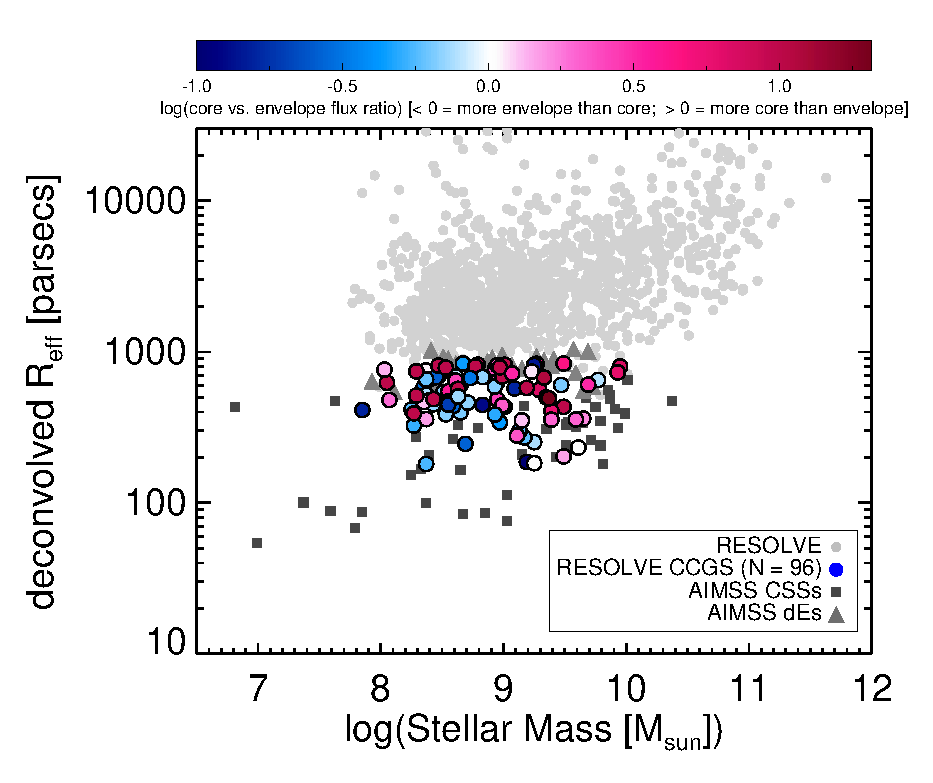
\includegraphics{Reff_Mstars.eps}
\caption{We plot here the deconvolved \Reff\ measurements for the entire RESOLVE sample, along with the CCSs of the AIMSS catalog. In grey are the RESOLVE (non-CCG) galaxies, which are plotted using their one component fit \Reff. The CCG sample is using the core \Reff\ of the two component fits, which is why they may appear separated from the full RESOLVE sample. The colors of the CCGs represent the logarithm of the flux ratio between the core and envelope. Galaxies with log(flux ratio) near 0 will have both a core and envelope, while galaxies with log(flux ratio) $\sim \pm 1$ will have more light in the core (+1) or envelope (-1).}
\label{fig:radius}
\end{center}
\end{figure*}

\section{Methods}
\label{methods}

\subsection{Photometry: galaxy colors, stellar and baryonic masses, and star formation rates}
\label{phot}
\noindent The RESOLVE survey overlaps with a number of photometric surveys, including GALEX $NUV$ \citep{Morrissey2007}, SDSS-DR8 $ugriz$ \citep{Aihara2011}, and UKIDSS $YHK$ and/or 2MASS $JHK$ \citep{Skrutskie2006}. We reprocess this photometric data to improve upon the standard SDSS data pipeline, as described in \citet{Eckert2015}. The main differences in this processing are (1) improved sky subtraction following Blanton et al. (2011) for SDSS photometry plus custom background subtraction for UKIDSS/2MASS, (2) the definition of elliptical apertures on the sum of the higher S/N $gri$ images to determine the PA and b/a ratio of the outer disk (if present), and (3) the application of the same apertures to all bands which allows us to measure magnitudes for galaxies that may not have been detected by automated survey pipelines, especially low surface brightness galaxies in 2MASS, UKIDSS, and GALEX. Then, total magnitudes are derived for each band using an exponential outer disk fit method, curve of growth method, or color correction method (see Figure 2 in \citet{Eckert2015}). 

Colors, stellar masses and fractional stellar mass growth rates (FSMGR) are then derived from these $NUVugrizYJHK$ magnitudes using the spectral energy distribution (SED) modeling code described in \citet{Kannappan2007}, \citet{Kannappan2009}, and \citet{Kannappan2013}. FSMGR is similar to a star formation rate, but it instead gives the ratio of stellar mass created in the last Gyr to the stellar mass previously existing. Therefore, an FSMGR of 1 means that the galaxy has doubled its stellar mass in the last Gyr.

The HI masses for RESOLVE are from the blind 21cm ALFALFA survey \citep{Haynes2011} and from new pointed observations with the GBT and Arecibo telescopes (Stark et al. in prep.). We use these masses along with the stellar masses computed in the SED models to estimate baryonic masses.

\subsection{Environmental Metrics}
\label{env}
\noindent RESOLVE is advantageous to this study because it offers excellent environment information, allowing us to search for CCGs in all environments including groups, clusters, walls, and filaments. We explore the environments of CCGs using two different metrics: the mass of their group halo and their distance to another galaxy. The group halo mass allows us to look for CCGs that are M32--Andromeda analogs where tidal stripping may be at play, or conversely look for CCGs in large groups where ram-pressure stripping could occur. The distance to neighboring galaxies lets us examine if interaction may occur or look for analogs of the isolated galaxies found by \citet{Huxor2013} and \citet{Paudel2014}.

Galaxy groups are identified using the friends-of-friends algorithm of \citet{Berlind2006}, and the masses of these group halos are calculated based on the observed total $r$-band luminosity of galaxies in each group using abundance matching, as described in \citet{Blanton2007}. More information on group identification can be found in \citet{Moffett2015}. The nearest neighbor distances are computed using the RA, Dec, and redshifts of each galaxy and along with spherical geometry principles. 

\subsection{Kinematics}
\label{kin}

\subsubsection{SOAR spectroscopy}
\noindent The RESOLVE survey gets the bulk of its spectroscopic data from the SOuthern Astrophysical Research (SOAR) Telescope, located at Cerro Tololo, Chile. We employ the Goodman Spectrograph, designed and built by UNC, along with RESOLVE's custom-built image slicer with 3 $1''$ slits to observe galaxies in both a broad setup and either an emission- or absorption-line kinematic setup. With this absorption-line setup, we are able to derive velocity dispersions. We use the highly-efficient 2100 l/mm VPH grating in order to cover a wavelength range 4858-5503\AA, which includes stellar absorption lines such as H$\beta$, the magnesium triplet, and Fe5270/5335. To achieve S/N $\sim$ 25 per \AA, we bin each central spectrum to \Reff.

The reduction process is as follows: we use standard IRAF tasks to perform bias and overscan subtraction, trimming of the science data to remove unnecessary spatial coverage, and flat fielding. We then use \texttt{LA\_COSMIC} \citep{vanDokkum2001} to clean cosmic rays from each science exposure. We next complete a wavelength calibration and transformation, and then perform object tracing and extraction into a 1D spectrum using the IRAF task apall. We lastly combine the individual exposures using the IRAF task scombine.

\subsubsection{Gemini-South spectroscopy}

\noindent A subset of the smallest galaxies in RESOLVE are observed with the Gemini-South IFU for their kinematics instead of SOAR. For this absorption-line setup, we use the B1200 grating in 1-slit mode to cover a spatial region of 3"$\times$5" and the spectral range 4200-5600\AA. The B1200 grating offers 0.9\AA\ resolution when binned spectrally by 2. We calculate our exposure times such that we achieve S/N $\sim$ 25 per \AA\, after binning by 2 in the spectral direction and summing the fibers out to \Reff.

The spectral reduction proceeds as follows. Using the standard IRAF Gemini-GMOS data packages, bias and overscan subtraction, spatial trimming, flat fielding and fiber identification are performed. We next use the GMOS package gemCRspec, a wrapper for \texttt{LA\_COSMIC}, to clean cosmic rays from each science exposure. We then correct the science frames for quantum efficiency differences between CCDs. Wavelength transformation, sky subtraction, and flux calibration are subsequently performed, and lastly, data cubes are made and summed. We then stack the individual fiber spectra out to \Reff\ to create a 1D spectrum for each galaxy that has S/N $\sim25$. More information on the data reduction for the Gemini GMOS IFU can be found in  Appendix A.

\subsubsection{Velocity Dispersion Extraction}

\noindent We then derive $\sigma$ from the both the SOAR and Gemini spectra using {\sc pPXF}, the penalized pixel fitting code from \citet{Cappellari2004}. This code fits a combination of high-resolution (FWHM $= 0.55$ \AA) ELODIE-based model spectra from \citet{Maraston2011} to the observed input spectrum, and determines a best fit solution for $\sigma$. A caveat to these fits is that they are not corrected for any stellar rotation, which will make absorption lines wider and thus skews the derived $\sigma$ values toward higher values depending on the amount of rotation in each galaxy. Future work will include implementing a stellar rotation subtraction routine for these fits, but preliminary testing by binning the spectra to $1''$ instead of to \Reff\ shows little change between the derived $\sigma$ values.

\begin{figure}[t]
\begin{center}
\includegraphics[scale=0.4]{rf0078ppxffit.eps}
\caption{Plotted here in black is a summed Gemini-South IFU spectrum for the CCG rf0078. Overplotted in red is the pPXF best fit model spectrum. The spectrum is zoomed-in to show the MgB triplet fit at $\sim 5275$ \AA.}
\label{fig:ppxffit}
\end{center}
\end{figure}

%%%%%%%%%%%%%%%%%%%%%%%%%%%%%%%
%%%%%%%%%%%%%%%%%%%%%%%%%%%%%%%
\section{Results}
\label{results}
\subsection{Colors and Star formation rates}

\begin{figure*}[t!]
\begin{center}
\includegraphics[scale=0.65]{sfr_mbary.eps}
\caption{\textbf{(a.)} On the left we plot the $u-r$ colors against stellar mass of CCGs with the entire RESOLVE sample. \textbf{(b.)} On the right we have plotted the FSMGR against baryonic mass for both the CCGs and entire RESOLVE sample. }
\label{fig:fsmgr}
\end{center}
\end{figure*}

\noindent We begin by examining the colors of the CCG sample. The left side of \autoref{fig:envplot} shows the $u-r$ colors of our CCG sample plotted against M$_{\star}$, compared to the RESOLVE sample as a whole. An unusual finding is that many CCGs live on the blue sequence, since most CSSs are typically thought of as being ``red and dead''. The right side of \autoref{fig:envplot} shows FSMGR vs. M$_{\rm bary}$ for the same objects. As with the colors, we find that many CCGs are forming stars at a rapid rate (FSMGR $\sim1$ means that the galaxy has doubled its mass in the last Gyr), again an unexpected finding which could indicate that some CCGs are still in the process of forming (if dissipatively formed) or relaxing (if a tidally-stripped remnant).

Looking now at the log(flux ratio values), we see that red sequence CCGs tend to be more core-dominated, while blue sequence CCGs tend to me more envelope-dominated. There also tends to be more core-dominated CCGs at lower FSMGR, while envelope-dominated CCGs reside at higher FSMGR. There is considerable scatter though, making these trends harder to qualify.


\subsection{Environments}
\noindent We investigate the distribution of CCGs throughout the cosmic web, and find that CCGs span a range of different environments (see \autoref{fig:envplot}). We see many CCGs residing in low mass groups, similar to the M32--Andromeda relationship, which suggests that tidal stripping could be at play. On the opposite end, we see several CCGs in massive group halos, and that these tend to be either core- or envelope dominated CCGs. This hints towards ram pressure stripping being at play in these environments, especially for those CCGs at larger distances from other galaxies. There are also many CCGs that are $>1$ Mpc away from another object in RA--Dec--redshift space, resembling the isolated cEs found by \citet{Huxor2013} and \citet{Paudel2014}, which may point to a dissipative formation scenario since there is no nearby object to have performed the stripping.
 

\begin{figure*}[t]
\begin{center}
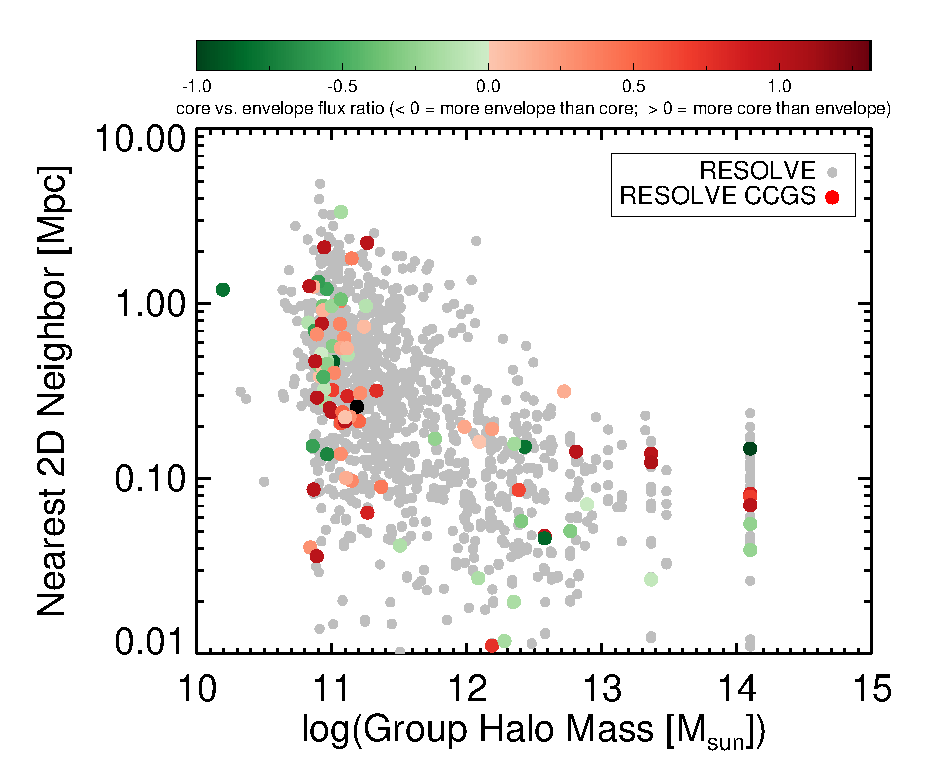
\includegraphics{nn_groupmass.eps}
\caption{We plot here the group halo mass against the nearest 3D neighbor for the RESOLVE survey and CCG sample. We see that CCGs live in a variety of environments, from extremely isolated (nearest neighbor $>$ 1 Mpc) to massive (M$_{\rm halo} \sim 10^{13}$ M$_{\odot}$) groups. There is no obvious trend into whether cores+envelopes and cores/envelopes preferentially live in different environments.}
\label{fig:envplot}
\end{center}
\end{figure*}

\subsection{Kinematics}
\label{kin}
\noindent We lastly investigate the kinematics of the CCG sample using the $\sigma$s derived from SOAR and Gemini telescope data. \autoref{fig:sigma} plots the $\sigma$-M$_{\star}$ relation for the 8 CCGs with $\sigma$ measurements along with the other 80+ RESOLVE galaxies with measured $\sigma$s. Galaxies with $\sigma$ offset to higher values point to tidal stripping occurring, since  they will have more  Conversely, $\sigma$s that lie on the trend may point dissipative formation occurring, since these will have formed similarly to normal elliptical galaxies.

We find that most of the CCGs tend to follow the dissipative formation track. However, there is one CCG with a core+envelope that lies close to M32, a tidally stripped cE, in the relation. We now take a closer look at this CCG, rf0492. This CCG lives on the red sequence, has an FSMGR$\sim 0.08$, and has a prominent core, and can be seen in the center image of \autoref{fig:pics}. Its nearest 3D neighbor is 2.63 Mpc away, making it fairly isolated, even though it lives in a group with halo mass = $10^{12.09}$ M$_{\odot}$. This could be an example of a CCG that was perturbed, perhaps even ram pressure stripped, as it fell into this larger group, causing gas to funnel to the center to create the core we see. 

\begin{figure*}[t!]
\begin{center}
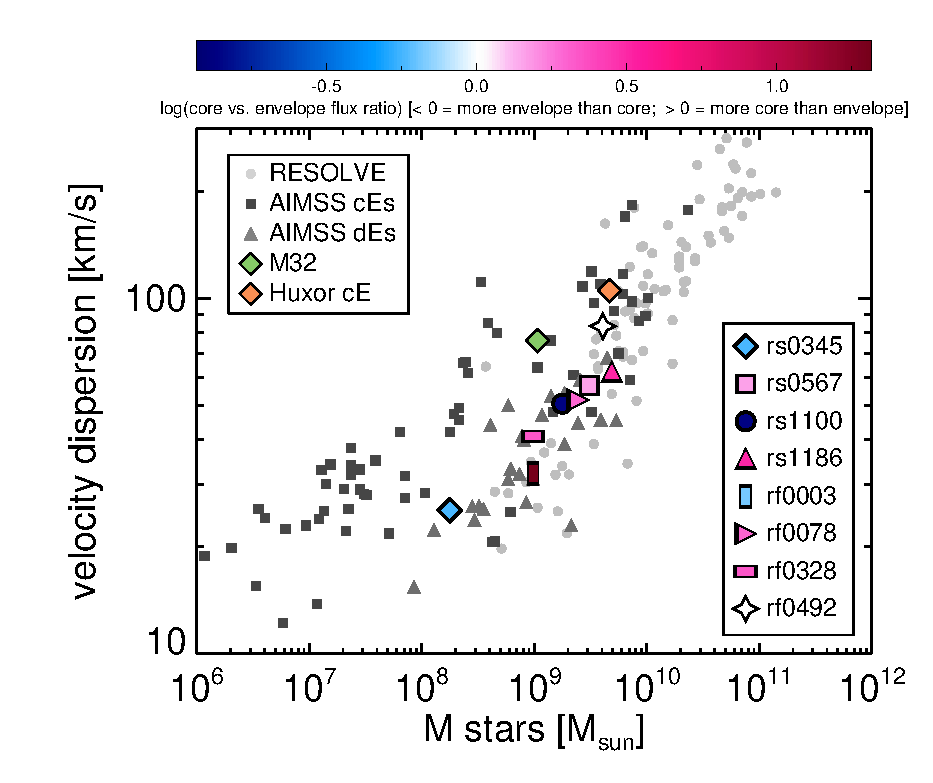
\includegraphics{faber-jackson_resolvesigmas.eps}
\caption{Here we plot the stellar mass vs. velocity dispersion ($\sigma$) for the RESOLVE sample, CCGs, and the CSSs of the AIMSS catalog. Most CCGs appear to be following the dissipative formation track.}
\label{fig:sigma}
\end{center}
\end{figure*}

%%%%%%%%%%%%%%%%%%%%%%%%%%%%%%%
%%%%%%%%%%%%%%%%%%%%%%%%%%%%%%%
%\section{CCG formation and evolution} %kind of like a discussion section



%%%%%%%%%%%%%%%%%%%%%%%%%%%%%%%
%%%%%%%%%%%%%%%%%%%%%%%%%%%%%%%
\section{Summary}
\label{conclusions}

\noindent In this paper we have examined the colors, FSMGR, environments, and kinematics of the 96 compact core galaxies (CCGs) in the RESOLVE survey. We have selected CCGs to have a seeing-deconvolved, core-only \Reff\ $<$ 800 pc, based on the sizes of the compact and dwarf ellipticals in the AIMSS catalog. We have quantified the amount of light in the cores and envelopes of each CCG by performing two component fits with \textsc{Galfit} and taking the logarithm of the ratio of the fluxes of the two different components. CCGs with more light in the envelope have log(flux ratio) $<$ 0 and are called ``envelope-dominated' CCGs. CCGs with more light in the core have log(flux ratio) $>$ 0 and are called ``core-dominated'' CCGs. CCGs with log(flux ratio) $\sim 0$ have both a bright core plus an extended envelope and are called ``core+envelope'' CCGs. Our main results can be summarized as follows:

\begin{enumerate}
\item \autoref{fig:radius} shows that both core- and envelope-dominated CCGs tend to be at the higher end of the \Reff\ values, while core+envelope CCGs tend to be the lower \Reff\ values. There also are more core-dominated CCGs at the higher M$_{\star}$ end while envelope-dominated CCGs tend to reside at low M$_{\star}$.

\item We find that many CCGs live on the blue sequence and are forming stars at a rapid rate (see \autoref{fig:fsmgr}), which could indicate that some CCGs are still in the process of forming (if dissipatively formed) or relaxing (if a tidally-stripped remnant).

\item We find that CCGs span a range of different environments (see \autoref{fig:envplot}). Many CCGs live in low mass groups, similar to the M32--Andromeda relationship, perhaps hinting at tidal stripping formation scenarios. Others live in massive group halos and tend to be either core- or envelope dominated CCGs, conversely hinting towards ram pressure stripping being at play. There are also many CCGs that are $>1$ Mpc away from another object in RA--Dec--redshift space, resembling the isolated cEs found by \citet{Huxor2013} and \citet{Paudel2014}, which may point to a dissipative formation scenario.

\item Using velocity dispersions ($\sigma$) derived from the SOAR and Gemini telescopes, we look for offsets in $\sigma$-M$_{\star}$ relation that could point to tidal stripping or dissipative formation scenarios (see \autoref{fig:sigma}). We find that CCGs tend to follow the dissipative formation track, however one CCG with a core+envelope lies close to M32, a tidally stripped cE, in the relation. 
\end{enumerate}

\section{Future Work}
\subsection{Gas Content}
\noindent The amount of neutral Hydrogen gas a CCG has may be able to give us insights into its evolution over time. For example, a CCG in a galaxy cluster with little HI gas may point towards ram pressure stripping being important. Combined with CCG colors and FSMGR, the gas content may be an important tool in determining the evolution of a CCG.

\subsection{Metallicities}
\noindent \citet{Janz2015} have shown that tidally-stripped CSSs are systematically offset to higher metal abundances. With the SOAR data we have in hand, we may be able to test this hypothesis for the CCG sample and use this method as another way to discern formation scenarios.

\acknowledgments{ \textit{Acknowledgements.}
  This work has been supported by funding from NSF grants AST-0955368 and OCI-1156614 and NASA grant HST-AR-12147.01-A. 
}

\bibliographystyle{apj}
\bibliography{library.bib}

\appendix


\end{document}
              
